\section{\label{sec:level1}Fabrication}
To observe typical characteristics of a SQUID such as the sinusoidal current-phase relationship (CPR), the niobium coherence length of $\xi$=40 nm  $^[$\citep{Clarke2005TheHandbook}${}^]$ must be approximately equal to the Dayem bridge dimensions $^[$\citep{Hao2015FabricationJunctions}${}^]$. In addition, the effective area of the superconducting ring is $^[$\citep{Troeman2007NanoSQUIDsConstrictions}${}^]$
\begin{equation}
\label{eq:effectivearea}
{A_{eff}} = {\Phi _0}/{B_0}
\end{equation}
where one period of the voltage-magnetic field (V-B) oscillation requires a magnetic field strength of ${B_0}$. The approximate value of $B_0$ for this fabricated SQUID is 2 mT.  

\begin{figure}[b]
\centering
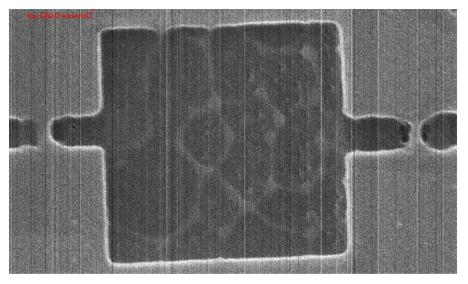
\includegraphics[width=0.4\textwidth]{B3after}
\caption{\label{fig:B3after}Fabricated SQUID on $Nb/Si$ chip. The loop is $\approx0.91\times {10^{ - 12}}$ m.The length ($l$) and width ($w$) of the left and right Dayem junctions are ($l$$\approx$ 80 nm, $w\approx$ 70 nm), ($l\approx$ 50 nm, $w$$\approx$ 50 nm), respectively.}
\end{figure}

The 50 nm thick $Nb$ film is coated on a 100 mm $Si$ wafer. Prior preliminary fabrication has been completed to produce a patterned chip the with electrical contact pads using polymethyl methacrylate (PMMA) resist and electron beam lithography (EBL) $^[$\citep{Granata2008AnApplications}${}^]$. The SQUID is created within the patterned section of the $Nb/Si$ chip by milling portions of the $Nb$ using a neon ($Ne$) focused ion beam (FIB). When the extraction field is applied the $Ne$ ions collect in approximately 10 nm cone at the point of the FIB needle $^[$\citep{Giannuzzi1999AScienceDirect_com}${}^]$. 

An acceleration voltage of $\approx$ 25 keV is used to fire the ions towards the sample. Sputtered particles referred to the injection of $Ne$ particles into the $Nb$ material when completing FIB milling
$^[$\citep{Giannuzzi1999AScienceDirect_com}${}^]$ and the FIB has Gaussian beam profile with a beam waist of $\approx$30 nm $^[$\citep{Troeman2007NanoSQUIDsConstrictions}${}^]$. Therefore there is an uncertainty associated with milling the $A_{eff}$ of the SQUID loop and the dimensions of the JJs. The detection of secondary electrons produced by the FIB enables image construction of the SQUID as shown in Fig.(\ref{fig:B3after}). The length ($l$) and width ($w$) of the left and right Dayem junctions are ($l$$\approx$ 80 nm, $w$$\approx$ 70 nm), ($l\approx$ 50 nm, $w$$\approx$ 50 nm), respectively. When the $l\ge3\xi$ the single-valued sinusoidal CPR is lost $^[$\citep{Troeman2007NanoSQUIDsConstrictions}${}^]$. The square superconducting loop has an $A_{eff}\approx0.91\times {10^{ - 12}}$ m. The sensitivity of the SQUID device is a function of the loop $A_{eff}$ $^[$\citep{Granata2008AnApplications}${}^]$.
